%===============================================================================================
%		Basic Terms and Domain Model
%===============================================================================================

\chapter{Basic Terms}
\label{sec:BasicTerms}

%-----------------------------------------------------------------------------------------------
%		Formal term definition
%-----------------------------------------------------------------------------------------------

\newcommand{\TERMtag}{\SpecialTermBasic{Tag}}
\newcommand{\TERMattribute}{\SpecialTermBasic{At\-tri\-but}}
\newcommand{\TERMmedium}{\SpecialTermBasic{Me\-di\-um}}
\newcommand{\TERMmedia}{\SpecialTermBasic{Me\-dia}}
\newcommand{\TERMdataBlock}{\SpecialTermBasic{Da\-ta\-block}}
\newcommand{\TERMdataBlocks}{\SpecialTermBasic{Da\-ta\-blocks}}
\newcommand{\TERMcontainer}{\SpecialTermBasic{Con\-tai\-ner}}
\newcommand{\TERMdataFormat}{\SpecialTermBasic{Da\-ta-\-For\-mat}}
\newcommand{\TERMmetadataFormat}{\SpecialTermBasic{Meta\-da\-ta-\-For\-mat}}
\newcommand{\TERMcontainerFormat}{\SpecialTermBasic{Con\-tai\-ner-\-For\-mat}}
\newcommand{\TERMfield}{\SpecialTermBasic{Field}}
\newcommand{\TERMfields}{\SpecialTermBasic{Fields}}
\newcommand{\TERMtransformation}{\SpecialTermBasic{Trans\-for\-mation}}
\newcommand{\TERMsubject}{\SpecialTermBasic{Sub\-ject}}
\newcommand{\TERMheader}{\SpecialTermBasic{Header}}
\newcommand{\TERMfooter}{\SpecialTermBasic{Footer}}
\newcommand{\TERMpayload}{\SpecialTermBasic{Payload}}
\newcommand{\TERMpadding}{\SpecialTermBasic{Pad\-ding}}

\newcommand{\TERMmediaStream}{\SpecialTermBasic{Media Stream}}
\newcommand{\TERMstreamingMedia}{\SpecialTermBasic{Strea\-ming Me\-dia}}

%-----------------------------------------------------------------------------------------------
%		Alle technischen Bezeichner
%-----------------------------------------------------------------------------------------------

%###########################
% Subsystem Bootstrap
%##########################
\newcommand{\SUBSBootstrap}{\texttt{Bootstrap}}

% --------------------------
% Komponente Kontext
% --------------------------
\newcommand{\COMPcontext}{\texttt{Easy\-Tag}}

%###########################
% Subsystem Low-Level
%##########################
\newcommand{\SUBSLowLevel}{\texttt{Container\- API}}
% --------------------------
% Komponente low level
% --------------------------
\newcommand{\COMPlowLevel}{\texttt{Container\- API}}
% --------------------------
% Komponente Data Part Management
% --------------------------
\newcommand{\COMPdataPartManagement}{\texttt{Data\-Blocks}}
% --------------------------
% Komponente Data Format Management
% --------------------------
\newcommand{\COMPdataFormatManagement}{\texttt{Data\-For\-mats}}
% --------------------------
% Komponente Media
% --------------------------
\newcommand{\COMPmedia}{\texttt{Me\-dia}}

% API
\newcommand{\IMediaAPI}{\texttt{IMedia\-API}}

\newcommand{\IMedium}{\texttt{IMedium}}
\newcommand{\FileMedium}{\texttt{File\-Medium}}
\newcommand{\InputStreamMedium}{\texttt{Input\-Stream\-Medium}}
\newcommand{\InMemoryMedium}{\texttt{In\-Memory\-Medium}}

\newcommand{\IMediumReference}{\texttt{IMedium\-Reference}}

\newcommand{\IMediumStore}{\texttt{IMedium\-Store}}
\newcommand{\MediumAction}{\texttt{Medium\-Action}}
\newcommand{\MediumReferenceRepository}{\texttt{Medium\-Reference\-Factory}}
\newcommand{\MediumChangeManager}{\texttt{Medium\-Change\-Manager}}
\newcommand{\MediumCache}{\texttt{Medium\-Cache}}
\newcommand{\MediumRegion}{\texttt{Medium\-Region}}

% Impl
\newcommand{\IMediumAccessor}{\texttt{IMediumAccessor}}

%###########################
% Subsystem High-Level
%##########################
\newcommand{\SUBSHighLevel}{\texttt{Metadata\- API}}
% --------------------------
% Komponente High Level
% --------------------------
\newcommand{\COMPhighLevel}{\texttt{Metadata\- API}}

%\newcommand{\COMPmetaData}{\texttt{Meta\-data}}
%\newcommand{\COMPmapping}{\texttt{Meta\-data\-Con\-ver\-sion}}
%\newcommand{\COMPvalidation}{\texttt{Vali\-da\-tion}}

%###########################
% Subsystem Techbase
%##########################
\newcommand{\SUBSTechBase}{\texttt{Technical\- Base}}
\newcommand{\COMPlogging}{\texttt{Log\-ging}}
\newcommand{\COMPextensionManagement}{\texttt{Ex\-ten\-sion\-Man\-age\-ment}}
\newcommand{\COMPconfiguration}{\texttt{Con\-fi\-gu\-ra\-tion}}
\newcommand{\COMPcomponentRegistry}{\texttt{Simple\-Com\-po\-nent\-Re\-gis\-try}}
\newcommand{\COMPutility}{\texttt{Utili\-ty}}

\newcommand{\ISimpleComponentRegistry}{\texttt{ISimple\-Com\-po\-nent\-Re\-gis\-try}}
\newcommand{\IComponentInterface}{\texttt{ICom\-po\-nent\-Inter\-face}}

\newcommand{\ComponentDescription}{Com\-po\-nent\-Descrip\-tion}
\newcommand{\ConfigProp}{\texttt{Abstract\-Con\-fig\-Param}}
\newcommand{\IConfigurable}{\texttt{ICon\-figu\-rable}}
\newcommand{\ConfigurationHandler}{\texttt{Con\-fig\-Hand\-ler}}
\newcommand{\IConfigurationChangeListener}{\texttt{ICon\-fig\-Change\-Listener}}

%###########################
% Subsystem Extension
%##########################
\newcommand{\SUBSExtension}{\texttt{Extension}}
%\newcommand{\COMPconcreteExtension}{\texttt{Con\-crete\-Ex\-ten\-sion}}

%===============================================================================================
%		Eigentlicher Start des Kapitels
%===============================================================================================

Here we define basic terms used throughout the whole design concept. Most of them come from \cite{MetaComp}, pages 19 to 29, where even more terms are defined.

All terms are based on a a domain model for container and metadata, as defined in \cite{MetaComp}. A domain model extended for our needs is shown in the following figure - it shows all relevant terms and their relations as an overview:
\OpenIssue{Add domain model figure}

%-----------------------------------------------------------------------------------------------

\section{Metadaten}
\label{sec:Metadata}

Metadata in this document is short for digital metadata that are not necessary to parse the actual described (audio, video or image) data. Metadata semantically and structurally describes other data. The goal of \LibName{} is especially reading of metadata for audio and video data sets, e.g. title, artist etc. The structure of metadata is defined by a \TERMmetadataFormat{}.

If it is specifically about technical metadata needed to parse a data structure, e.g. in the container header,  we call it \emph{Parsing Metadata}.

%-----------------------------------------------------------------------------------------------

\section{\TERMdataFormat{}e, \TERMmetadataFormat{}e und \TERMcontainerFormat{}e}
\label{sec:DataFormats}

A \TERMdataFormat{} specifies the structure and interpretation
of data: Which bytes of which value and order have what kind of meaning?
Usually, a data format describes how a consecutive block of bytes (i.e. a \TERMdataBlock{}) is built up by a number of so-called \TERMfield{} or child \TERMdataBlock{}.

\TERMmetadataFormat{}s are data formats that define the structure of digital metadata. Examples include:
\begin{itemize}
	\item ID3v1
	\item ID3v2.3
	\item APEv1
	\item MPEG-7
	\item RDF/XML
	\item VorbisComment
	\item and others ...
\end{itemize}

\TERMcontainerFormat{}s are special \TERMdataFormat{}s optimized for storing, transporting, editing and seeking multimedia \TERMpayload{} data. Examples are:
\begin{itemize}
	\item MP3
	\item Ogg
	\item TIFF
	\item QuickTime
	\item JPEG 2000
	\item PDF
	\item and others...
\end{itemize}

An example for other \TERMdataFormat{}s is HTML. It is neither called a \TERMmetadataFormat{} nor a \TERMcontainerFormat{}. XML is a \TERMdataFormat{} that itself can be used to define further XML \TERMdataFormat{}s. Some XML \TERMdataFormat{}s are \TERMmetadataFormat{}s, e.g. MPEG-7, MPEG-21 or P\_Meta.

%-----------------------------------------------------------------------------------------------

\section{\TERMtransformation{}en}
\label{sec:DataTransformations}

A \TERMdataFormat{} may define \TERMtransformation{}s. A \TERMtransformation{} describes a way how read or to be written data needs to be transformed to fulfill specific needs. You can envision this as kind of encoding of the data. In contrast to the fixed data format specification which describes in detail how binary data is coded and needs to be interpreted, \TERMtransformation{}s are optional features that are dynamically applied to certain areas of the data. Partly, \TERMtransformation{}s can also be defined by users of the data. Examples are the \TERMtransformation{}s defined by ID3v2: Unsynchronization, Encryption and Compression.

%-----------------------------------------------------------------------------------------------

\section{\TERMdataBlocks{}}
\label{sec:DataBlocks}

A \TERMdataBlock{} is a sequence of bytes that together form a logical unit in terms of the underlying \TERMdataFormat{}. Each \TERMdataBlock{} belongs to exactly one \TERMdataFormat{}. It can be assigned a current length in bytes. There are several concrete types of \TERMdataBlock{}s that are described in the following sections.

%***********************************************************************************************

\subsection{\TERMcontainer{}: \TERMpayload{}, \TERMheader{}, \TERMfooter{}}
\label{sec:Containers}

An important type of \TERMdataBlock{} is a \TERMcontainer{}: It consists of an optional \TERMheader{}, exactly one \TERMpayload{} and maybe an optional \TERMfooter{}. All of these are \emph{child} \TERMdataBlock{}s, meaning that a \TERMcontainer{} is built-up by these three blocks.

\TERMcontainer{}s are a common concept for container and metadata formats: The \TERMheader{} describes the \TERMcontainer{} in terms of its length, size and other properties. The \TERMpayload{} contains the interesting data, e.g. the multimedia data to be played. A \TERMfooter{} allows for backwards or reverse reading. Most of the time, a \TERMcontainer{} is typed with its id, i.e. the id defines the kind and structure of data block. Furthermore, most of \TERMdataFormat{}s specify a general structure of a \TERMcontainer{} so that user-defined new \TERMcontainer{}s can be added, i.e. the format is extensible.

%***********************************************************************************************

\subsection{\TERMtag{}}
\label{sec:Tag}

A \TERMtag{} is a special \TERMcontainer{} whose purpose is to store metadata. It can either belong to a standalone \TERMmetadataFormat{} ore to a more general \TERMcontainerFormat{}. Especially audio metadata formats use this term when talking about such a \TERMdataBlock{} in a file or \TERMmediaStream{}, e.g. the ID3 or APE \TERMtag{}s.

The following figure shows the basic structure of a \TERMtag{}, showing other basic terms:

\begin{figure}[H]
	\centering
		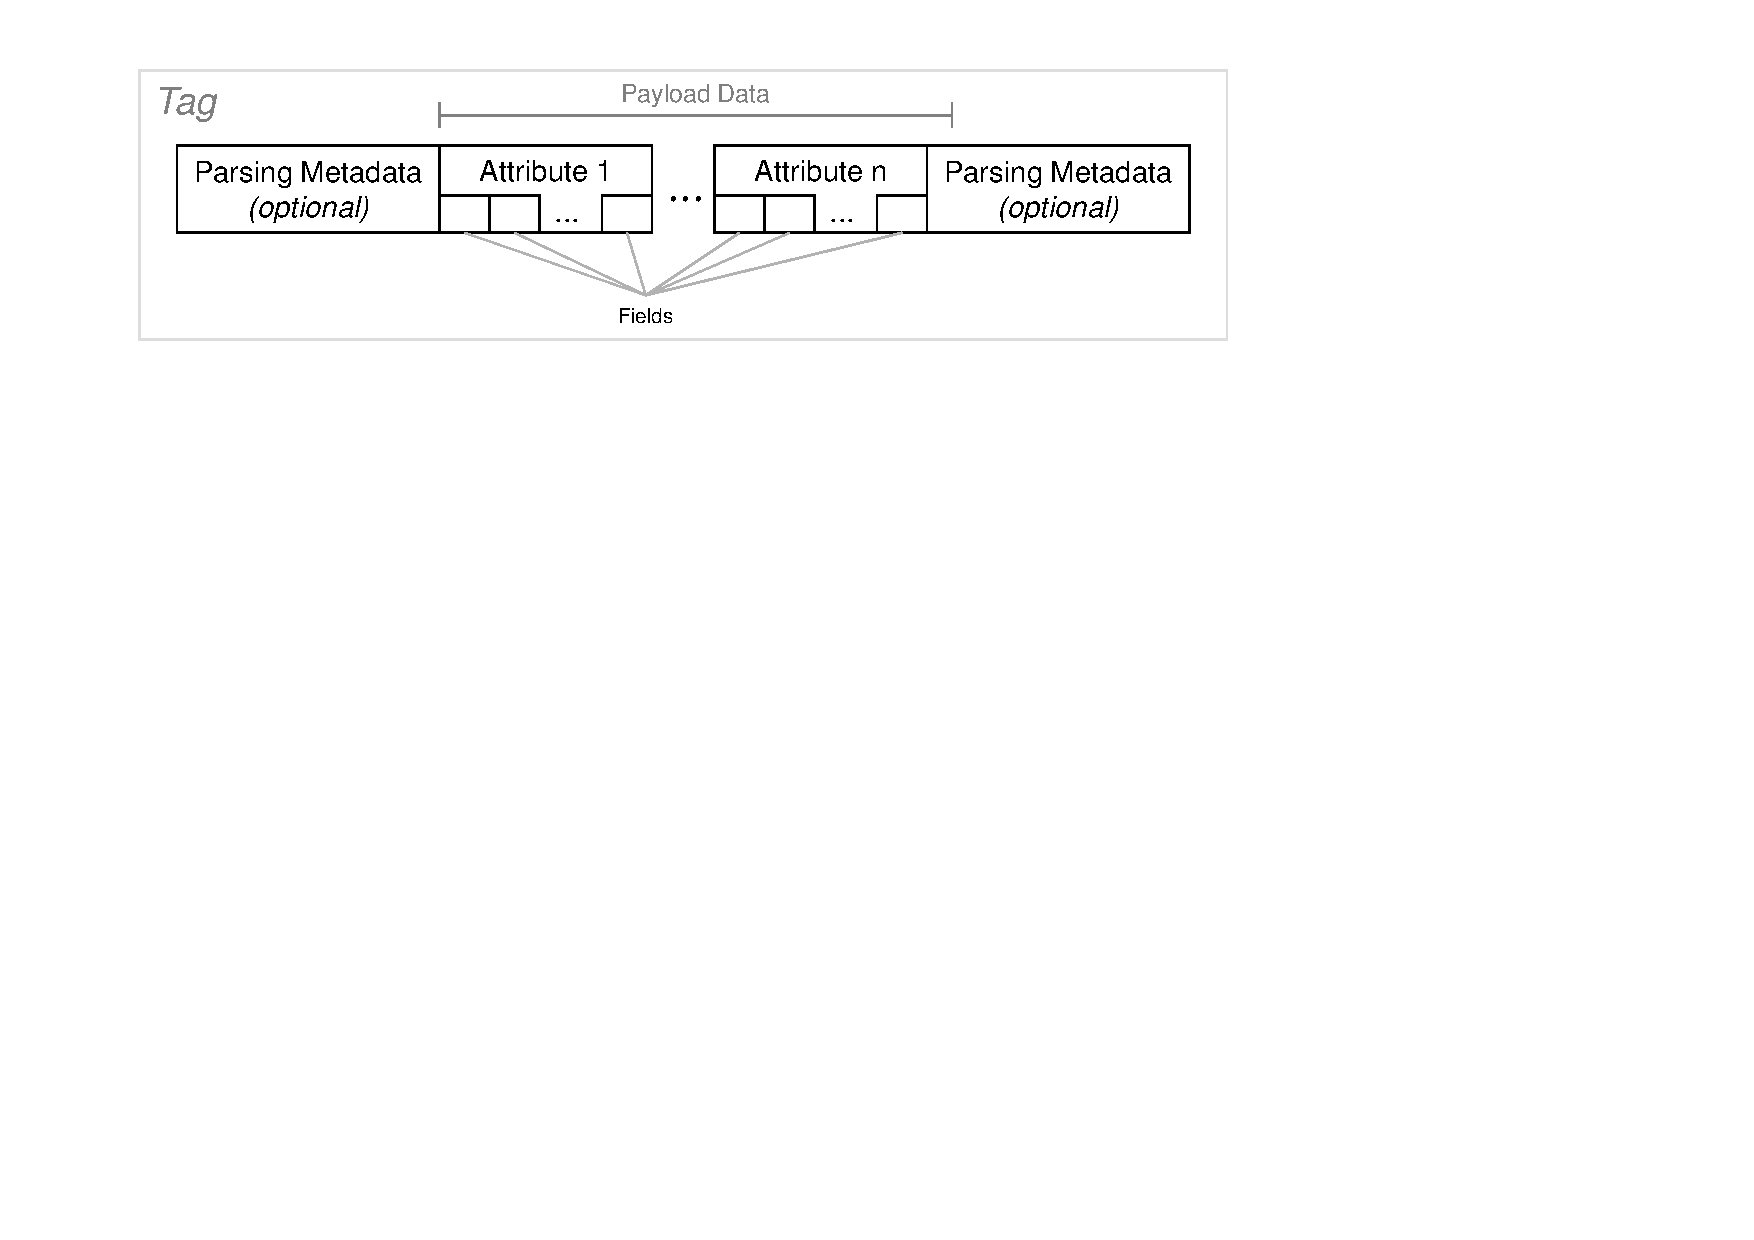
\includegraphics[width=1.00\textwidth]{Figures/Part_I/I_3_TagStructure.pdf}
		\caption{Structure of a \TERMtag{}}
	\label{fig:5_3_SCH_Tag}
\end{figure}

The most important parts of a \TERMtag{} are the \TERMattribute{}s.

%***********************************************************************************************

\subsection{\TERMattribute{}}
\label{sec:Attribute}

An \TERMattribute{} is a part of a \TERMtag{} that contains the valuable metadata information in a key-value manner. Common examples are artist, title, album, composer etc. of a piece of audio. Often, an \TERMattribute{} is also a \TERMcontainer{} in a sense that it has a \TERMheader{}. The \TERMheader{} may help to define the type (artist, title, album) of the \TERMattribute{} as well as the size of the payload. The \TERMpayload{} contains the actual information in an encoded way, e.g. the name of the artist or title of the piece of audio.

Most of the \TERMattribute{}s have a simple main value that can be given. However, there are also more complex \TERMattribute{}s that consists of many values in form of child \TERMdataBlock{}s or \TERMfield{}s.

In each metadata format, an \TERMattribute{} has a specific name, e.g.:
\begin{itemize}
	\item ID3v1, Lyrics3: Field
	\item ID3v2: Frame
	\item APE: Item
	\item Matroska: SimpleTag
	\item VorbisComment: User Comment
\end{itemize}

In \TERMcontainerFormat{}s, the \TERMattribute{}s are often \TERMcontainer{}s defined by the \TERMcontainerFormat{}.

%***********************************************************************************************

\subsection{\TERMfield{}s}
\label{sec:Fields}

A \TERMfield{} is a sequence of bits that together have a specific meaning in a given \TERMdataFormat{}. The \TERMdataFormat{} describes how a specific \TERMdataBlock{} is built up by a specific sequence of \TERMfield{}s. A \TERMfield{} has a range of possible values and
interpretations of these values. Often, one part of the value range is defined as ``reserved'' to ensure a bit of flexibility in extending the data format.

%-----------------------------------------------------------------------------------------------

\subsection{\TERMsubject{}}
\label{sec:Subject}

A \TERMsubject{} represents a thing a \TERMtag{} describes, i.e. a part of a file, a piece of audio, a web resource or even a thing existing in reality. Often, a \TERMtag{} contains metadata for the current \TERMmedium{}, not explicitly referring to a more specific \TERMsubject{}.

%-----------------------------------------------------------------------------------------------

\section{\TERMmedium{}}
\label{sec:Medium}

A medium is the place where data \TERMdataBlock{}s are physically persisted and accessible. This may be a file, a \TERMmediaStream{} or even plain memory.

%###############################################################################################
%###############################################################################################
%
%		File end
%
%###############################################################################################
%###############################################################################################